%%%%%%%%%%%%%%%%%%%%%%%%%%%%%%%%%%%%%%%%%%%%%%%%%%%%%%%%%%%%%%%%%%
%%%%%%%% ICML 2017 EXAMPLE LATEX SUBMISSION FILE %%%%%%%%%%%%%%%%%
%%%%%%%%%%%%%%%%%%%%%%%%%%%%%%%%%%%%%%%%%%%%%%%%%%%%%%%%%%%%%%%%%%

% Use the following line _only_ if you're still using LaTeX 2.09.
%\documentstyle[icml2017,epsf,natbib]{article}
% If you rely on Latex2e packages, like most moden people use this:
\documentclass{article}

% use Times
\usepackage{times}
% For figures
\usepackage{graphicx} % more modern
%\usepackage{epsfig} % less modern
%\usepackage{subfigure} 
\usepackage{caption}
\usepackage{subcaption}

% For citations
\usepackage{natbib}

% AMS stuff
\usepackage{amsmath, amsthm, amssymb}
\newtheorem{theorem}{Theorem}
\newtheorem{lemma}{Lemma}
\newtheorem{cor}{Corollary}

% For algorithms
\usepackage{algorithm}
\usepackage{algorithmic}

% As of 2011, we use the hyperref package to produce hyperlinks in the
% resulting PDF.  If this breaks your system, please commend out the
% following usepackage line and replace \usepackage{icml2017} with
% \usepackage[nohyperref]{icml2017} above.
\usepackage{hyperref}

% Packages hyperref and algorithmic misbehave sometimes.  We can fix
% this with the following command.
\newcommand{\theHalgorithm}{\arabic{algorithm}}

% Employ the following version of the ``usepackage'' statement for
% submitting the draft version of the paper for review.  This will set
% the note in the first column to ``Under review.  Do not distribute.''
\usepackage{icml2017} 

% Employ this version of the ``usepackage'' statement after the paper has
% been accepted, when creating the final version.  This will set the
% note in the first column to ``Proceedings of the...''
%\usepackage[accepted]{icml2017}


% The \icmltitle you define below is probably too long as a header.
% Therefore, a short form for the running title is supplied here:
\icmltitlerunning{ Active Deep Learning}

\begin{document} 

\twocolumn[
\icmltitle{ Active Deep Learning}

% It is OKAY to include author information, even for blind
% submissions: the style file will automatically remove it for you
% unless you've provided the [accepted] option to the icml2017
% package.

% list of affiliations. the first argument should be a (short)
% identifier you will use later to specify author affiliations
% Academic affiliations should list Department, University, City, Region, Country
% Industry affiliations should list Company, City, Region, Country

% you can specify symbols, otherwise they are numbered in order
% ideally, you should not use this facility. affiliations will be numbered
% in order of appearance and this is the preferred way.

\begin{icmlauthorlist}
\icmlauthor{Ozan Sener}{to}
\icmlauthor{Silvio Savarese}{to}
\end{icmlauthorlist}

\icmlaffiliation{to}{Department of Computer Science, Stanford University, CA, US}

\icmlcorrespondingauthor{Ozan Sener}{ozan@cs.stanford.edu}

% You may provide any keywords that you 
% find helpful for describing your paper; these are used to populate 
% the "keywords" metadata in the PDF but will not be shown in the document
\icmlkeywords{boring formatting information, machine learning, ICML}

\vskip 0.3in
]

% this must go after the closing bracket ] following \twocolumn[ ...

% This command actually creates the footnote in the first column
% listing the affiliations and the copyright notice.
% The command takes one argument, which is text to display at the start of the footnote.
% The \icmlEqualContribution command is standard text for equal contribution.
% Remove it (just {}) if you do not need this facility.

%\printAffiliationsAndNotice{}  % leave blank if no need to mention equal contribution
\printAffiliationsAndNotice{} % otherwise use the standard text.
%\footnotetext{hi}

\begin{abstract} 
Abstract.
\end{abstract} 

\section{Introduction}
\begin{itemize}
\item To the best of our knowledge, the first empirical negative result on uncertainty based active learning for deep learning
\item An active learning query algorithm designed and analyzed specifically for convolutional neural networks.
\item Joint treatment of semi-supervised learning and active learning in the context of deep-learning. 
\item Simple and very effective algorithm for active learning in deep learning outperforming all state-of-the-art competitors
\end{itemize}

\section{Related Work}

\subsection{Active Learning}
Classical survey of classical algorithms \cite{settles2010active}

Some early information theoretical methods for queries \cite{mackay1992information}

Another class is query-by-commitee \cite{mccallumzy1998employing, freund1997selective}

Convex optimization combining diversity and uncertainity \cite{elhamifar2013convex}



 One of the first theoretical results \cite{dasgupta2004analysis} showing negative results except average case.

 First agnostic non-Bayesial algorithm but not computationally applicable \cite{balcan2009agnostic}

In a very recent result, \cite{huang2015efficient} building on ideas, give a new efficient agnostic active learning algorithm that is both general and aggressive. Uncertainty based and would not scale to deep-learning scale

\subsection{Active Deep Learning with CNNs}
Recent deep learning one \cite{wang2016cost} worse than semi-supervised, actually semi supervised

One important class is uncertainty based selection \cite{tong2001support,lewissequential,joshi2009multi} like entropy \cite{joshi2009multi} geometric metric for SVM \cite{tong2001support}

\subsection{Semi-Supervised Deep Learning}

Improved GAN \cite{salimans2016improved} \cite{ali} \cite{bigan} \cite{ladder}


\subsection{Problem of Subset Selection}
Active domain adaptation based on distance \cite{BerlindU15} only for kNN classifier

Very similar algorithm for a similar problem \cite{wei2013using} unsupervised subset selection

Core-set for SVM \cite{tsang2005core}

Core-set for k-Means and k-Medians \cite{har2005smaller}

Submodularity in hyphotesis(query space) for a set-cover problem \cite{guillory2010interactive}

Submodularity specifically for k-NN and Naive Bayes \cite{wei2015submodularity}

Stochastic extension of set-cover further used for active learning with noisy variables \cite{golovin2011adaptive}

Use GP to model expected improvement \cite{kapoor2007active}.

Extend uncertanity to information density \cite{li2013adaptive}

Extending any bayesian optimization to multiple instance \cite{wang2016parallel}

Extend SVM active learning combining a metric with diversity \cite{brinker2003incorporating}.

Bayesian optimiziation to optimize future error \cite{roy2001toward}
 


\section{Problem Definition}
We are interested in $C$ class classification problem defined over a space $\mathcal{X}$ and a label space  $\mathcal{Y}=\{1,\ldots,C\}$. We also consider a loss function $l(\cdot,\cdot;\mathbf{w}):\mathcal{X}\times \mathcal{Y} \rightarrow \mathcal{R}$ parametrized over the hyphotesis class ($\mathbf{w}$), e.g.\ parameters of the deep learning algorithm.

We consider a large collection of data points which are sampled iid over the space  $\mathcal{Z}=\mathcal{X}\times\mathcal{Y}$ as \mbox{$\{\mathbf{x}_i,y_i\}_{i \in [n]} \sim p_\mathcal{Z}$}. We further consider an initial pool of data-points chosen iid among them as \mbox{$\mathbf{s}^0=\{s(i) \in [n]\}_{i \in [m]}$}. 

In our setting, an active learning algorithm has only access to $\{\mathbf{x}_i\}_{i \in [n]}$ and $\{y_{s(j)}\}_{j \in [m] }$. In other words, it can not see the labels of all data points except the initial sub-sampled pool. It is also given a budget $b$ of queries to ask to an oracle and a (semi)supervised learning algorithm $A_{\mathbf{s}}$ which outputs a set of parameters $\mathbf{w}$ given a labelled set $\mathbf{s}$. The active learning with a pool problem can simply be defined as
\begin{equation}
\min_{\mathbf{s}^1 : |\mathbf{s}^1| \leq b} E_{\mathbf{x},y \sim p_\mathcal{Z}} [l(\mathbf{x},y; A_{\mathbf{s}^0 \cup \mathbf{s}^1})]
\end{equation}
In other words, an active learning algorithm can choose $b$ extra points and get it labelled by an oracle to minimize the future expected loss.

There are a few differences between our formulation and the classical definition of active learning. Classical methods consider the case the budget is 1 as $b=1$ but a single point has negligible effect in a deep learning regime. It is also very common to consider multiple round of this game as;
\begin{equation}
\min_{\mathbf{s}^{k+1} : |\mathbf{s}^{k+1}| \leq b} E_{\mathbf{x},y \sim p_\mathcal{Z}} [l(\mathbf{x},y; A_{\mathbf{s}^{0} \cup \ldots, \mathbf{s}^{k+1}})]
\end{equation}
Although it is more realistic, analysis is typically trickier in such a setting. Hence, we consider the greedy version and try to solve the single round of labelling. In practice, we use multiple rounds by solving each single

\section{Limitations of the existing methods}
\noindent\textbf{Hypothesis:} \emph{Deep learning algorithms results in an inaccurate estimate of uncertainty hence the uncertainty based methods fail.}

This is very easy to experiment by simply replacing the uncertainty estimates in active learning with oracle ground truth loss. In other words, we replace the uncertainty with $l(\mathbf{x}_i,y_i,A_{\mathbf{s}^0})$. Hence, instead of sampling data points using estimated uncertainty, we sample them using the ground truth loss.

\begin{figure}[ht]

\includegraphics[width=\columnwidth]{placeholder1.jpg}
\caption{Comparison of iid. sampling and active learning with oracle loss information. This figure suggests that even with oracle loss estimates, uncertainty based active learning algorithms would not work in deep learning regime.}
\end{figure}

Hence as a negative result, the hypothesis is rejected. We need to search for a different reason. One interesting way to qualitatively study the behavior is looking at the embedding plots.

\begin{figure}[ht]

\includegraphics[width=\columnwidth]{placeholder1.jpg}
\caption{tSNE embeddings for data points with their actual loss. The embedding suggest that sampling based on loss estimates and/or uncertainty would result in a bias and the resulting samples would not cover the space.}
\end{figure}

In conclusion, we suspect that the critical property of an active learning algorithm in deep learning regime is covering the space efficiently. In the next section, we discuss such an algorithm.

\section{Active Learning as a Space Covering}
Using the heuristic of covering the space efficiently, here we explain our algorithm. Our algorithm is simply based on the \emph{k-Center} problem (min-max facility location problem \cite{cook}) which can be defined in our setting as;
\begin{equation}
\min_{\mathbf{s}^1} \max_i \min_{j \in \mathbf{s}^1 \cup \mathbf{s}^0} \Delta(\mathbf{x}_i,\mathbf{x}_j)
\end{equation}
which simply minimizes the maximum distance between any point and its nearest labelled neighbor. 

Unfortunately this problem is NP-Hard \cite{cook}. However, it is possible to obtain a $2-OPT$ solution very efficiently using a greedy as Algorithm~\ref{alg:greedy}.

\begin{algorithm}[ht]
   \caption{k-Center-Greedy}
   \label{alg:greedy}
\begin{algorithmic}
   \STATE {\bfseries Input:} data $\mathbf{x}_i$, existing pool $\mathbf{s}^0$ and a budget $b$
    \STATE Initialize $\mathbf{s}=\mathbf{s}^0$
   \REPEAT
   \STATE $u=\arg\max_{i \in [n] \setminus \mathbf{s}} \min_{j \in \mathbf{s}} \Delta(\mathbf{x}_i, \mathbf{x}_j)$
   \UNTIL {$|\mathbf{s}|<b+|\mathbf{s}^0|$}
   \STATE {\bfseries return} $\mathbf{s} \setminus \mathbf{s}^0$
\end{algorithmic}
\end{algorithm}

Given any desired solution $\delta$, we can check its feasibility (i.e.\ is it $\min_{\mathbf{s}^1} \max_i \min_{j \in \mathbf{s}^1 \cup \mathbf{s}^0} \Delta(\mathbf{x}_i,\mathbf{x}_j) \leq \delta$) by constructing an mixed integer program and checking is it feasible or not. Hence, a straight-forward algorithm to choose this k-Center problem is doing a binary search between the result of the greedy algorithm and its half since that region guaranteed to include the optimal solution. By constructing this algorithm, we also consider one of the weakness of k-Center algorithm -robustness-. To make the k-Center problem robust, we assume a upper on the number of outliers $\Xi$ such that our algorithm can choose to not cover at most $\Xi$ data points. This mixed integer program can be written as combination of constraints:

\begin{equation}
\begin{aligned}
Feasible(b,\mathbf{s}^0,\delta, \Xi):  &\sum_j  u_j = |\mathbf{s}^0|+ b \\
&\sum_j \omega_{i,j} = 1 \quad \forall  i \\
   &\omega_{i,j} = \xi_{i,j} \quad  \forall i,j \mid   \Delta(\mathbf{x}_i,\mathbf{x}_j)  > \delta \\
   &\omega_{i,j} \leq u_j \quad \forall  i \\
   &u_j =1 \quad \forall j\in \mathbf{s}^0 \\
   & \sum_{i,j} \xi_{i,j} \leq \Xi \\
   & u_i, \omega_{i,j}, \xi_{i,j} \in \{0,1\}
\end{aligned}
\end{equation}

In this formulation, $u_i$ is 1 if $i^{th}$ data point chosen as center and $0$ otherwise, $\omega_{i,j}$ is $1$ if $i^{th}$ point is covered by $j^{th}$ point and $\xi_{i,j}$ is 1 if $i^{th}$ point is an outlier and included in $j^{th}$ point without the $\delta$ constraint. We further visualize these variables in a diagram in Figure~\ref{mip}.

\begin{figure}[h]
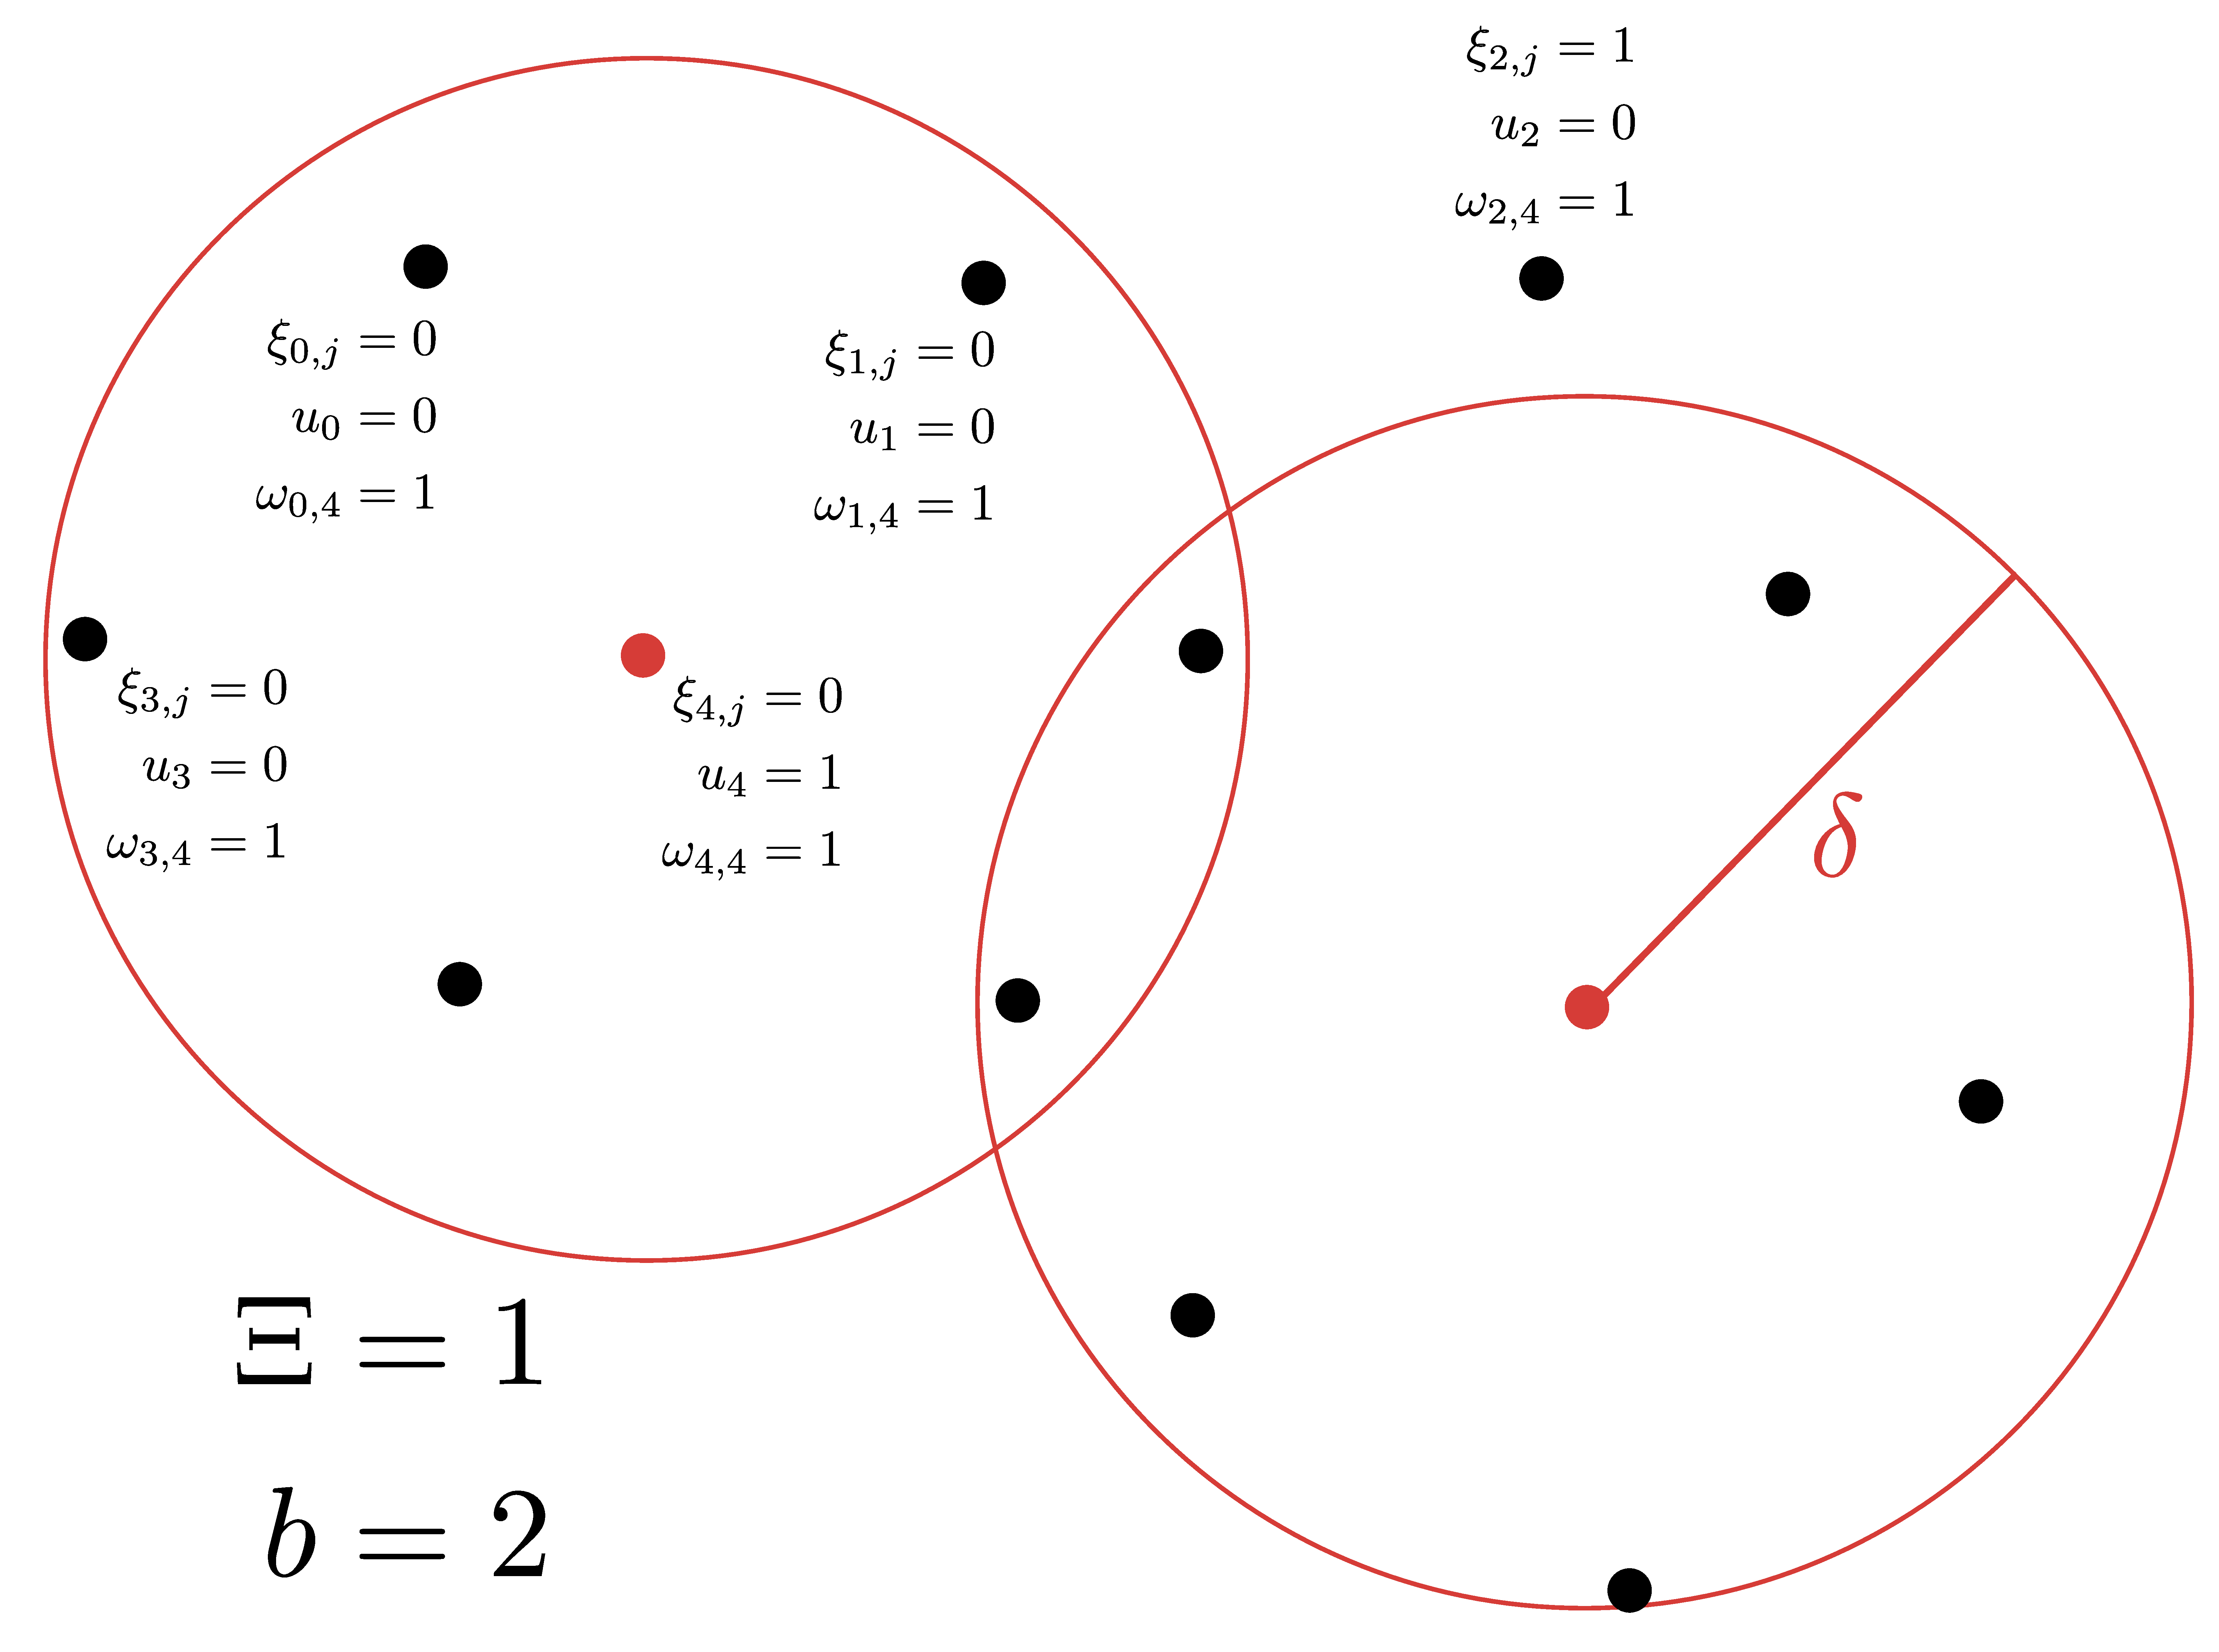
\includegraphics[width=\columnwidth]{mip.pdf}
\caption{Visualizations of the variables in the mixed integer program.}
\label{mip}
\end{figure}

We solve this mixed integer program using Gurobi\cite{gurobi} software toolbox. We further give details of the binary search procedure using this mixed integer program in algorithmic form in Algorithm~\ref{alg:bin}. 

\begin{algorithm}[tb]
   \caption{Robust k-Center}
   \label{alg:bin}
\begin{algorithmic}
   \STATE {\bfseries Input:} data $\mathbf{x}_i$, existing pool $\mathbf{s}^0$, budget $b$ and outlier bound $\Xi$
   \STATE {\bfseries Initialize} $\delta_{2-OPT}$ = k-Center-Greedy($\mathbf{x}_i, \mathbf{s}^0, b$)
   \STATE $lb=\frac{\delta_{2-OPT}}{2}$, $ub=\delta_{2-OPT}$
   \REPEAT
   \IF {$Feasible(b, \mathbf{s}^0,\frac{lb+ub}{2},\Xi)$}
   \STATE $ub=\max_{i,j \mid  \Delta(\mathbf{x}_i,\mathbf{x}_j) \leq \frac{lb+ub}{2}}  \Delta(\mathbf{x}_i,\mathbf{x}_j) $
   \ELSE
   \STATE $lb=\min_{i,j \mid   \Delta(\mathbf{x}_i,\mathbf{x}_j) \geq \frac{lb+ub}{2}}  \Delta(\mathbf{x}_i,\mathbf{x}_j) $
    \ENDIF
   \UNTIL{$ub = lb$}
      \STATE {\bfseries return} $\{i\ st.\ u_i=1\}$
\end{algorithmic}
\end{algorithm}
\section{Semi-Supervised Active Learning}
\section{Experimental Results}

\begin{figure*}
    \centering
    \begin{subfigure}[b]{0.3239\textwidth}
        
\includegraphics[width=\textwidth]{placeholder1.jpg}
        \caption{MNIST}
    \end{subfigure}
    ~ %add desired spacing between images, e. g. ~, \quad, \qquad, \hfill etc. 
      %(or a blank line to force the subfigure onto a new line)
    \begin{subfigure}[b]{0.3239\textwidth}
        
\includegraphics[width=\textwidth]{placeholder1.jpg}
        \caption{Cifar-10}
    \end{subfigure}
    ~ %add desired spacing between images, e. g. ~, \quad, \qquad, \hfill etc. 
    %(or a blank line to force the subfigure onto a new line)
    \begin{subfigure}[b]{0.3239\textwidth}
        
\includegraphics[width=\textwidth]{placeholder1.jpg}
        \caption{Cifar-100}
    \end{subfigure}
    \caption{Results on Active Learning without Semi-Supervision}\label{fig:resnosemi}
\end{figure*}

\begin{figure*}
    \centering
    \begin{subfigure}[b]{0.3239\textwidth}
        
\includegraphics[width=\textwidth]{placeholder1.jpg}
        \caption{MNIST}
    \end{subfigure}
    ~ %add desired spacing between images, e. g. ~, \quad, \qquad, \hfill etc. 
      %(or a blank line to force the subfigure onto a new line)
    \begin{subfigure}[b]{0.3239\textwidth}
        
\includegraphics[width=\textwidth]{placeholder1.jpg}
        \caption{Cifar-10}
    \end{subfigure}
    ~ %add desired spacing between images, e. g. ~, \quad, \qquad, \hfill etc. 
    %(or a blank line to force the subfigure onto a new line)
    \begin{subfigure}[b]{0.3239\textwidth}
        
\includegraphics[width=\textwidth]{placeholder1.jpg}
        \caption{Cifar-100}
    \end{subfigure}
    \caption{Results on Active Learning with Semi-Supervision}\label{fig:ressemi}
\end{figure*}


\begin{figure}[h]

\includegraphics[width=\columnwidth]{placeholder1.jpg}
\caption{Effect of approximation in set-cover problem.}
\label{mip}
\end{figure}


\begin{figure}[h]

\includegraphics[width=\columnwidth]{placeholder1.jpg}
\caption{Test error vs $\gamma$}
\label{mip}
\end{figure}




\section{Analysis of Algorithm}

\begin{lemma}
Softmax function defined over $C$ class is  Lipschitz continuous with $\lambda=\frac{\sqrt{C-1}}{C}$
\end{lemma}

\begin{lemma}
A convolutional neural network with $n_c$ convolutional (with max-pool and ReLU) and $n_{fc}$ fully connected layers defined over C class with loss function defined as 2-norm between softmax and class probability is $(\mathcal{N}(\gamma/C,\mathcal{Z},|\cdot|_2),  \frac{\sqrt{C-1}}{C} \alpha^{n_c+n_{fc}})$ robust.
\end{lemma}


\begin{theorem}
Given $n$ i.i.d. samples drawn from $p(\mathbf{x},y)$ as $\{\mathbf{x}_i,y_i\}_{i\in[n]}$, and $m$ points $\{ s(i) \in [N]\}_{\i \in [m]}$. If,
\begin{enumerate}
\item  $\{x_{s(i)}\}_{i \in [m]}$ is $\bar{\epsilon}-cover$ for  $\{\mathbf{x}_i\}_{i\in[n]}$
\item Algorithm $A_s$ is $(K,\epsilon(s))$ robust
\item Loss function is $\lambda$-Lipschitz continous
\item $l_{emp}(A_s,x)=0\quad \forall x \in s$
\end{enumerate}
With probability at least $(1-\gamma)$,
\[
E[l(A_s,z)] \leq \frac{n-m}{n} \lambda \tilde{\epsilon} + \epsilon(s) + L \sqrt{\frac{2K\ln 2 + 2\ln (1/\gamma)}{n}}
\]
\label{mainthm}
\end{theorem}



\clearpage

\bibliography{active_adversarial}
\bibliographystyle{icml2017}

\clearpage

\begin{proof}
It is easy to show that for any differentiable function $f:\mathbb{R}^n\rightarrow\mathbb{R}^m$,

\[
\left \|f(x)-f(y)\right \|_2 \leq \left \|J\right \|^*_F \left \|x-y\right\|_2 \, \, \forall x,y\in\mathbb{R}^n
\]
where $\left \|J\right \|^*_F = \max\limits_{x} \left \|J\right \|_F$ and $J$ is the jacobian matrix of $f(x)$ wrt $x$.

Softmax function is defined as
\[
f(x)_i = \frac{\exp(x_i)}{\sum\limits_{j=1}^{C}\exp(x_j)} = p_i(x), \, i={1,2,...C}
\]
For brevity, We will denote $p_i(x)$ as $p_i$. The jacobian matrix for some $x$ will be,
\[
J = \begin{bmatrix} p_1(1-p_1) & p_1p_2  & ... & p_1p_K \\
p_2p_1 & p_2(1-p_2)  & ...  & p_2p_K \\
... & ... & ... & ...  \\
p_{K}p_{1} & p_{K}p_{2}  & ...  & p_{K}(1-p_{K})
\end{bmatrix}
\]
Now, Frobenius norm of above matrix will be,
\[
\left \| J \right \|_F = \sqrt{\sum\limits_{i=1}^{K}\sum\limits_{j=1 \\ i\neq j}^{K}p_{i}^{2}p_{j}^{2} + \sum\limits_{i=1}^{K} p_i^2(1-p_i^2)}
\]
It is straightforward to show that $p_i = \frac{1}{K}$ is the optimal solution for $\left \| J \right \|^{*}_F = \max\limits_{x}\left \| J \right \|_F $ Hence,


Putting $p_i = \frac{1}{K}$ in above equation of $\left \| J \right \|_F$, we get $\left \| J \right \|^{*}_F = \frac{\sqrt{K-1}}{K}$

\end{proof}


\begin{proof}
Consider two inputs $\mathbf{x}_u$ and $\mathbf{x}_v$, such that their representation at layer $d$ is $\mathbf{x}_u^d$ and $\mathbf{x}_v^d$. Consider any conv+max pool+relu layer, if $\sum_i w_{i,j} \leq \alpha \forall j$, we can simply state
\[
|\mathbf{x}_u^d - \mathbf{x}_v^d| \leq  \alpha |\mathbf{x}_u^{d-3} - \mathbf{x}_v^{d-3}|
\] 
Here, we used $|a-b| \leq |\max(0, a) - \max(0,a)|$ and the fact that max pool layer can be written as a convolutional layer such that only one weight is 1 and others are 0. For fully connected layers, we can also use the same argument and show;
\[
|\mathbf{x}_u^d - \mathbf{x}_v^d| \leq  \alpha |\mathbf{x}_u^{d-1} - \mathbf{x}_v^{d-1}|
\] 
For soft-max layer, we need to use the Lemma \ref{softmax_lip} as,
\[
|\mathbf{x}_u^d - \mathbf{x}_v^d| \leq  \frac{\sqrt{C-1}}{C} |\mathbf{x}_u^{d-1} - \mathbf{x}_v^{d-1}|
\] 
Hence,
\[
|l(\mathbf{x}_u) - l(\mathbf{x}_v)| \leq   \frac{\sqrt{C-1}}{C} \alpha^{n_c+n_{fc}}  |\mathbf{x}_u-\mathbf{x}_v|
\]
\end{proof}

\begin{proof}
\begin{small}
We will start with
\[
\begin{aligned}
&\left|E[l(A_s,z)] - \frac{1}{n}\sum_i l(A_s,x_i) \right| \\
&\leq \left|\sum_{j} E[l(A_s,z)|z \in C_j] \mu_{j} -  \sum_{j} E[l(A_s,z)|z \in C_j] \frac{|N_j|}{n} \right| \\
 &+  \left|\sum_{j} E[l(A_s,z)|z \in C_j] \frac{|N_j|}{n}  - \frac{1}{n}\sum_i l(A_s,x_i)\right| \\
  &\leq\left|\sum_{j} E[l(A_s,z)|z \in C_j] (\mu_{j} -   \frac{|N_j|}{n}) \right|\\
 &+\frac{1}{n} \left|\sum_j \sum_{i \in N_j} E[l(A_s,z)|z \in C_j]  - l(A_s,x_i)\right| \\
   &\leq \left|\sum_{j} E[l(A_s,z)|z \in C_j] (\mu_{j} -   \frac{|N_j|}{n})\right| +\epsilon(s)  \\
 \end{aligned}
\]
Now, we will use the zero-loss of the classifier with Lipschitz continuity as;
\[
\begin{aligned}
\left|\frac{1}{n}\sum_i l(A_s,x_i) \right| &= \left|\frac{1}{n}\sum_{j \notin {s(i)}_{i\in [M]}} l(A_s,x_i)  \right| \\
&\leq  \frac{1}{n}\sum_{j \notin {s(i)}_{i\in [M]}} \lambda  \left| \mathbf{x}_i - \mathbf{x}_k\right | \leq \frac{n-m}{n} \lambda \tilde{\epsilon}
\end{aligned}
\]
Combining both,
\[
\begin{aligned}
&E[l(A_s,z)] \leq  \left|E[l(A_s,z)] - \frac{1}{n}\sum_i l(A_s,x_i) \right|  \\ &+ \left|\frac{1}{n}\sum_i l(A_s,x_i) - \frac{1}{m}\sum_i l(A_s,x_{s(i)}) \right| \\
&\leq \left|\sum_{j} E[l(A_s,z)|z \in C_j] (\mu_{j} -   \frac{|N_j|}{n})\right| +\epsilon(s) + \frac{n-m}{n} \lambda \tilde{\epsilon}
\end{aligned}
\]
\end{small}
We finally use Breteganolle-Huber-Carol inequality (\emph{cf} Proposition A6.6 of \cite{wellner}):
\[
E[l(A_s,z)] \leq \frac{n-m}{n} \lambda \tilde{\epsilon} + \epsilon(s) + L \sqrt{\frac{2K\ln 2 + 2\ln (1/\gamma)}{n}}
\]
\end{proof}

\begin{cor}
If the conditions in Theorem \ref{mainthm} satisfied except $4$ and $l_{emp}(A_s,x)=0\quad \forall x \in \overline{s}$, with probability at least $(1-\gamma)$,
\begin{small}
\[
E[l(A_s,z)] \leq \frac{n-|\overline{s}|}{n} \lambda \tilde{\epsilon} + \epsilon(s) + L \sqrt{\frac{2K\ln 2 + 2\ln (1/\gamma)}{n}} + \frac{2|s|L}{n}  
\]
\end{small}
\end{cor}
\begin{proof}
\[
\begin{aligned}
&\left|\frac{1}{n}\sum_i l(A_s,x_i) \right| \leq \left|\frac{1}{n}\sum_{j \notin {s(i)}_{i\in [M]}} l(A_s,x_i)  \right| +  \left|\frac{1}{n}\sum_{j \notin\overline{s}} l(A_s,x_i)  \right| \\
&\leq  \frac{1}{n}\sum_{j \notin {s(i)}_{i\in [M]}} \lambda  \left| \mathbf{x}_i - \mathbf{x}_k\right | +\frac{n-|\overline{s}|}{n}L \\
&\leq \frac{n-m}{n} \lambda \tilde{\epsilon}
\end{aligned}
\]
\end{proof}


\end{document} 
